\documentclass[11pt]{exam}

\usepackage{amssymb, amsmath, amsthm, mathrsfs, multicol, graphicx}
\usepackage{tikz, pgfplots}


\def\d{\displaystyle}
\def\?{\reflectbox{?}}
\def\b#1{\mathbf{#1}}
\def\f#1{\mathfrak #1}
\def\c#1{\mathcal #1}
\def\s#1{\mathscr #1}
\def\r#1{\mathrm{#1}}
\def\N{\mathbb N}
\def\Z{\mathbb Z}
\def\Q{\mathbb Q}
\def\R{\mathbb R}
\def\C{\mathbb C}
\def\F{\mathbb F}
\def\A{\mathbb A}
\def\X{\mathbb X}
\def\E{\mathbb E}
\def\O{\mathbb O}
\def\pow{\mathscr P}
\def\inv{^{-1}}
\def\nrml{\triangleleft}
\def\st{:}
\def\~{\widetilde}
\def\rem{\mathcal R}
\def\iff{\leftrightarrow}
\def\Iff{\Leftrightarrow}
\def\and{\wedge}
\def\And{\bigwedge}
\def\AAnd{\d\bigwedge\mkern-18 mu\bigwedge}
\def\Vee{\bigvee}
\def\VVee{\d\Vee\mkern-18 mu\Vee}
\def\imp{\rightarrow}
\def\Imp{\Rightarrow}
\def\Fi{\Leftarrow}


\def\bar{\overline}

%\pointname{pts}
\pointsinmargin
\marginpointname{pts}
\marginbonuspointname{ bns pts}

\addpoints
\pagestyle{headandfoot}
%\printanswers


\header{MATH 131}{\bf\large Learning Target 17 Quiz}{Fall 2025}
\runningfooter{}{}{Version \version}
\extrafootheight{-.45 in}

\begin{document}
\def\version{A}
%space for name
\noindent {\large\bf Name:} \underline{\hspace{2.5 in}}
\vskip 1em

\begin{questions}
\question The \emph{velocity} $v(t)$, in feet per second, of a model rocket, $t$ seconds after launch, has graph shown below.  

\begin{center}
    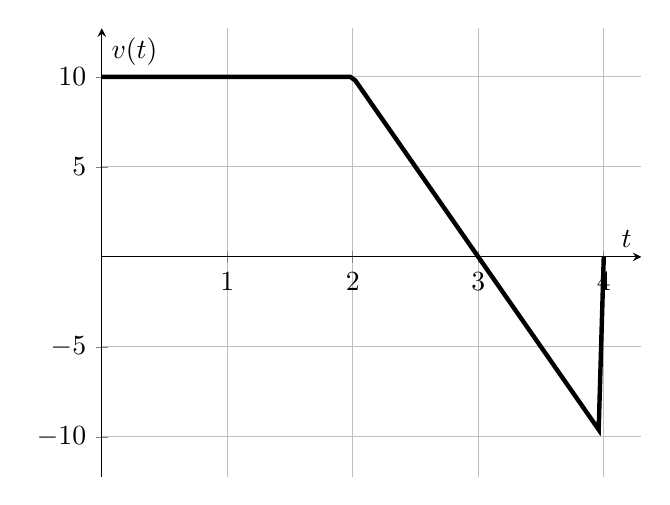
\begin{tikzpicture}[
      declare function={
        func(\x) = ( \x < 2) * (10) + and(\x >= 2, \x < 4) * ((-10*\x)+30);
      }
    ]
      \begin{axis}[
        axis x line=middle, axis y line=middle, ymin=-12.2, ymax=12.7, xmin=0, xmax=4.3, xlabel=$t$, ylabel=$v(t)$, grid=major
      ]
        \addplot [domain=0:4, samples=100, ultra thick]{func(x)};
      \end{axis}
    \end{tikzpicture}
\end{center}
\begin{parts}
\part Find the total distance traveled by the rocket in the first three seconds (between seconds 0 and 3).  Briefly explain how you found your answer.
\vfill
\part Find the total \emph{change in position} of the rocket in the first \emph{four} seconds (between seconds 0 and 4).  Explain why this is less than the distance traveled in the first three seconds.
\vfill
\end{parts}
\end{questions}



\newpage

\def\version{B}
%space for name
\noindent {\large\bf Name:} \underline{\hspace{2.5 in}}
\vskip 1em

\begin{questions}
\question The \emph{velocity} $v(t)$, measured in feet per second, of a bungee-jumper, $t$ seconds after he jumps, has graph shown below.  

\begin{center}
    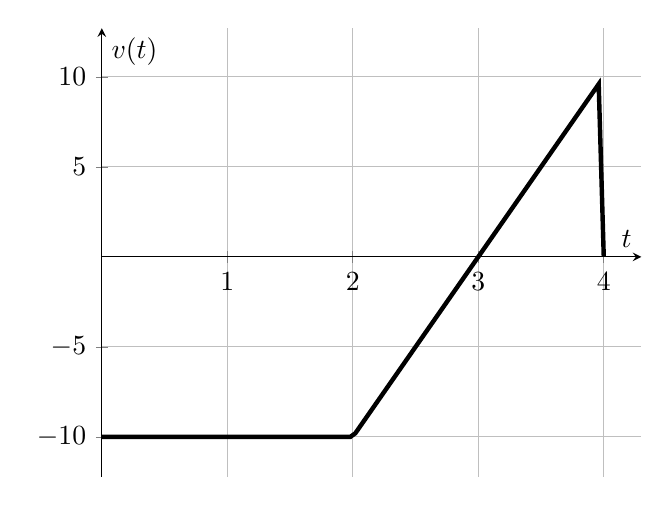
\begin{tikzpicture}[
      declare function={
        func(\x) = ( \x < 2) * (-10) + and(\x >= 2, \x < 4) * ((10*\x)-30);
      }
    ]
      \begin{axis}[
        axis x line=middle, axis y line=middle, ymin=-12.2, ymax=12.7, xmin=0, xmax=4.3, xlabel=$t$, ylabel=$v(t)$, grid=major
      ]
        \addplot [domain=0:4, samples=100, ultra thick]{func(x)};
      \end{axis}
    \end{tikzpicture}
\end{center}
\begin{parts}
\part Find the total distance traveled by the bungee-jumper in the first three seconds (between seconds 0 and 3).  Briefly explain how you found your answer.
\vfill
\part Find the total \emph{change in position} of the bungee-jumper in the first \emph{four} seconds (between seconds 0 and 4).  Explain why this is negative and how it relates to the distance traveled from the previous question.
\vfill
\end{parts}
\end{questions}

\newpage

\def\version{C}
%space for name
\noindent {\large\bf Name:} \underline{\hspace{2.5 in}}
\vskip 1em

\begin{questions}
\question The \emph{velocity} $v(t)$, in feet per second, of a model rocket launched from the top of a skyscraper, $t$ seconds after launch, has graph shown below.  

\begin{center}
    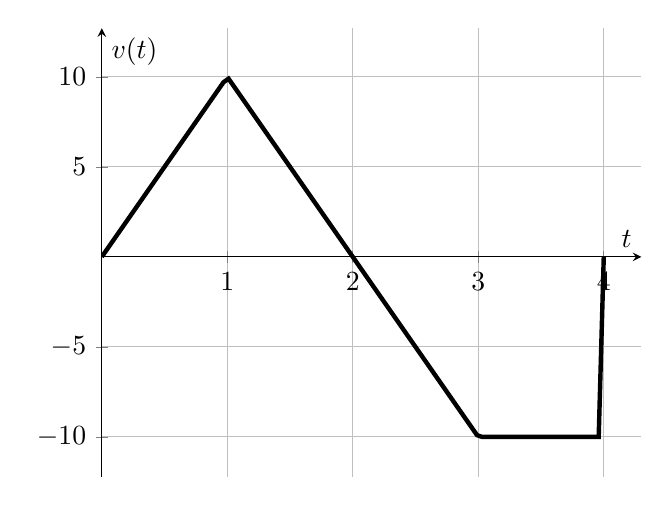
\begin{tikzpicture}[
      declare function={
        func(\x) = ( \x < 1) * (10*\x) + and(\x >= 1, \x < 3) * (-10*\x+20) + and(\x >= 3, \x < 4) * (-10) ;}
    ]
      \begin{axis}[
        axis x line=middle, axis y line=middle, ymin=-12.2, ymax=12.7, xmin=0, xmax=4.3, xlabel=$t$, ylabel=$v(t)$, grid=major
      ]
        \addplot [domain=0:4, samples=100, ultra thick]{func(x)};
      \end{axis}
    \end{tikzpicture}
\end{center}
\begin{parts}
\part Find the total distance traveled by the rocked in the first two seconds (between seconds 0 and 2).  Briefly explain how you found your answer.
\vfill
\part Find the total \emph{change in position} of the rocked in the first \emph{four} seconds (between seconds 0 and 4).  Explain why this is less than the distance traveled in the first two seconds.
\vfill
\end{parts}
\end{questions}


\newpage

\def\version{D}
%space for name
\noindent {\large\bf Name:} \underline{\hspace{2.5 in}}
\vskip 1em


\begin{questions}
\question The \emph{velocity} $v(t)$, in feet per second, of an amusement park ride that propels riders forwards and backwards along a straight path, $t$ seconds after it starts, has graph shown below.  

\begin{center}
    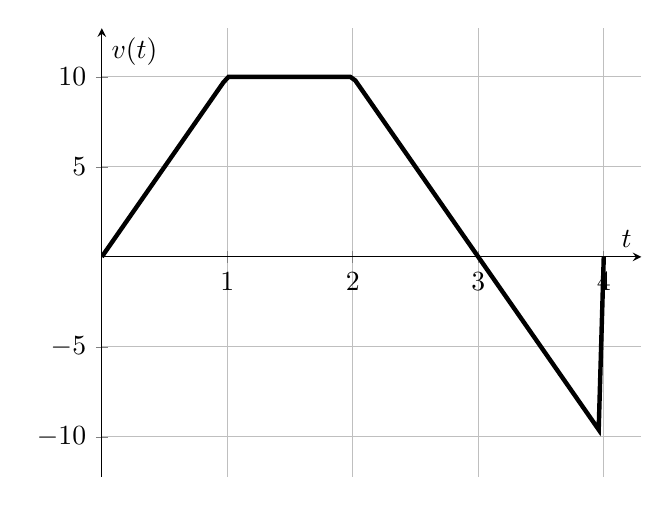
\begin{tikzpicture}[
      declare function={
        func(\x) = ( \x < 1) * (10*\x) + and(\x >= 1, \x < 2) * (10) + and(\x >= 2, \x < 4) * ((-10*\x)+30) ;
      }
    ]
      \begin{axis}[
        axis x line=middle, axis y line=middle, ymin=-12.2, ymax=12.7, xmin=0, xmax=4.3, xlabel=$t$, ylabel=$v(t)$, grid=major
      ]
        \addplot [domain=0:4, samples=100, ultra thick]{func(x)};
      \end{axis}
    \end{tikzpicture}
\end{center}
\begin{parts}
\part Find the total distance traveled by the ride in the first three seconds (between seconds 0 and 3).  Briefly explain how you found your answer.
\vfill
\part Find the total \emph{change in position} of the ride in the first \emph{four} seconds (between seconds 0 and 4).  Explain why this is less than the distance traveled in the first three seconds.
\vfill
\end{parts}
\end{questions}

\end{document}
